% Options for packages loaded elsewhere
\PassOptionsToPackage{unicode}{hyperref}
\PassOptionsToPackage{hyphens}{url}
\documentclass[
]{article}
\usepackage{xcolor}
\usepackage{amsmath,amssymb}
\setcounter{secnumdepth}{-\maxdimen} % remove section numbering
\usepackage{iftex}
\ifPDFTeX
  \usepackage[T1]{fontenc}
  \usepackage[utf8]{inputenc}
  \usepackage{textcomp} % provide euro and other symbols
\else % if luatex or xetex
  \usepackage{unicode-math} % this also loads fontspec
  \defaultfontfeatures{Scale=MatchLowercase}
  \defaultfontfeatures[\rmfamily]{Ligatures=TeX,Scale=1}
\fi
\usepackage{lmodern}
\ifPDFTeX\else
  % xetex/luatex font selection
\fi
% Use upquote if available, for straight quotes in verbatim environments
\IfFileExists{upquote.sty}{\usepackage{upquote}}{}
\IfFileExists{microtype.sty}{% use microtype if available
  \usepackage[]{microtype}
  \UseMicrotypeSet[protrusion]{basicmath} % disable protrusion for tt fonts
}{}
\makeatletter
\@ifundefined{KOMAClassName}{% if non-KOMA class
  \IfFileExists{parskip.sty}{%
    \usepackage{parskip}
  }{% else
    \setlength{\parindent}{0pt}
    \setlength{\parskip}{6pt plus 2pt minus 1pt}}
}{% if KOMA class
  \KOMAoptions{parskip=half}}
\makeatother
\usepackage{color}
\usepackage{fancyvrb}
\newcommand{\VerbBar}{|}
\newcommand{\VERB}{\Verb[commandchars=\\\{\}]}
\DefineVerbatimEnvironment{Highlighting}{Verbatim}{commandchars=\\\{\}}
% Add ',fontsize=\small' for more characters per line
\newenvironment{Shaded}{}{}
\newcommand{\AlertTok}[1]{\textcolor[rgb]{1.00,0.00,0.00}{\textbf{#1}}}
\newcommand{\AnnotationTok}[1]{\textcolor[rgb]{0.38,0.63,0.69}{\textbf{\textit{#1}}}}
\newcommand{\AttributeTok}[1]{\textcolor[rgb]{0.49,0.56,0.16}{#1}}
\newcommand{\BaseNTok}[1]{\textcolor[rgb]{0.25,0.63,0.44}{#1}}
\newcommand{\BuiltInTok}[1]{\textcolor[rgb]{0.00,0.50,0.00}{#1}}
\newcommand{\CharTok}[1]{\textcolor[rgb]{0.25,0.44,0.63}{#1}}
\newcommand{\CommentTok}[1]{\textcolor[rgb]{0.38,0.63,0.69}{\textit{#1}}}
\newcommand{\CommentVarTok}[1]{\textcolor[rgb]{0.38,0.63,0.69}{\textbf{\textit{#1}}}}
\newcommand{\ConstantTok}[1]{\textcolor[rgb]{0.53,0.00,0.00}{#1}}
\newcommand{\ControlFlowTok}[1]{\textcolor[rgb]{0.00,0.44,0.13}{\textbf{#1}}}
\newcommand{\DataTypeTok}[1]{\textcolor[rgb]{0.56,0.13,0.00}{#1}}
\newcommand{\DecValTok}[1]{\textcolor[rgb]{0.25,0.63,0.44}{#1}}
\newcommand{\DocumentationTok}[1]{\textcolor[rgb]{0.73,0.13,0.13}{\textit{#1}}}
\newcommand{\ErrorTok}[1]{\textcolor[rgb]{1.00,0.00,0.00}{\textbf{#1}}}
\newcommand{\ExtensionTok}[1]{#1}
\newcommand{\FloatTok}[1]{\textcolor[rgb]{0.25,0.63,0.44}{#1}}
\newcommand{\FunctionTok}[1]{\textcolor[rgb]{0.02,0.16,0.49}{#1}}
\newcommand{\ImportTok}[1]{\textcolor[rgb]{0.00,0.50,0.00}{\textbf{#1}}}
\newcommand{\InformationTok}[1]{\textcolor[rgb]{0.38,0.63,0.69}{\textbf{\textit{#1}}}}
\newcommand{\KeywordTok}[1]{\textcolor[rgb]{0.00,0.44,0.13}{\textbf{#1}}}
\newcommand{\NormalTok}[1]{#1}
\newcommand{\OperatorTok}[1]{\textcolor[rgb]{0.40,0.40,0.40}{#1}}
\newcommand{\OtherTok}[1]{\textcolor[rgb]{0.00,0.44,0.13}{#1}}
\newcommand{\PreprocessorTok}[1]{\textcolor[rgb]{0.74,0.48,0.00}{#1}}
\newcommand{\RegionMarkerTok}[1]{#1}
\newcommand{\SpecialCharTok}[1]{\textcolor[rgb]{0.25,0.44,0.63}{#1}}
\newcommand{\SpecialStringTok}[1]{\textcolor[rgb]{0.73,0.40,0.53}{#1}}
\newcommand{\StringTok}[1]{\textcolor[rgb]{0.25,0.44,0.63}{#1}}
\newcommand{\VariableTok}[1]{\textcolor[rgb]{0.10,0.09,0.49}{#1}}
\newcommand{\VerbatimStringTok}[1]{\textcolor[rgb]{0.25,0.44,0.63}{#1}}
\newcommand{\WarningTok}[1]{\textcolor[rgb]{0.38,0.63,0.69}{\textbf{\textit{#1}}}}
\usepackage{longtable,booktabs,array}
\newcounter{none} % for unnumbered tables
\usepackage{calc} % for calculating minipage widths
% Correct order of tables after \paragraph or \subparagraph
\usepackage{etoolbox}
\makeatletter
\patchcmd\longtable{\par}{\if@noskipsec\mbox{}\fi\par}{}{}
\makeatother
% Allow footnotes in longtable head/foot
\IfFileExists{footnotehyper.sty}{\usepackage{footnotehyper}}{\usepackage{footnote}}
\makesavenoteenv{longtable}
\usepackage{graphicx}
\makeatletter
\newsavebox\pandoc@box
\newcommand*\pandocbounded[1]{% scales image to fit in text height/width
  \sbox\pandoc@box{#1}%
  \Gscale@div\@tempa{\textheight}{\dimexpr\ht\pandoc@box+\dp\pandoc@box\relax}%
  \Gscale@div\@tempb{\linewidth}{\wd\pandoc@box}%
  \ifdim\@tempb\p@<\@tempa\p@\let\@tempa\@tempb\fi% select the smaller of both
  \ifdim\@tempa\p@<\p@\scalebox{\@tempa}{\usebox\pandoc@box}%
  \else\usebox{\pandoc@box}%
  \fi%
}
% Set default figure placement to htbp
\def\fps@figure{htbp}
\makeatother
\setlength{\emergencystretch}{3em} % prevent overfull lines
\providecommand{\tightlist}{%
  \setlength{\itemsep}{0pt}\setlength{\parskip}{0pt}}
\usepackage{bookmark}
\IfFileExists{xurl.sty}{\usepackage{xurl}}{} % add URL line breaks if available
\urlstyle{same}
\hypersetup{
  pdftitle={PENTAGON: Can Closed-Loop LLM Reasoning Achieve Autonomous Multi-Tool Cybersecurity Assessment?},
  pdfauthor={Obi Ebuka David; Sayed Erfan Arefin},
  pdfkeywords={\xmpquote{autonomous penetration
testing}, \xmpquote{large language model agents}, \xmpquote{closed-loop
reasoning}, \xmpquote{vulnerability assessment}, \xmpquote{ablation
study}, \xmpquote{OWASP}},
  hidelinks,
  pdfcreator={LaTeX via pandoc}}

\title{PENTAGON: Can Closed-Loop LLM Reasoning Achieve Autonomous
Multi-Tool Cybersecurity Assessment?}
\author{Obi Ebuka David\footnote{Department of Computer Science,
  University of Dayton, USA. Corresponding author ---
  davidobi023@gmail.com} \and Sayed Erfan Arefin\footnote{Department of
  Computer Science, University of Dayton, USA.}}
\date{}

\begin{document}
\maketitle
\begin{abstract}
We investigate whether a large language model, operating in a closed
reasoning loop over real cybersecurity tools, can produce an autonomous
vulnerability assessment that approaches human-expert coverage at a
fraction of the time and cost. We focus on the \textbf{assessment
regime} (find + reason + adapt), explicitly orthogonal to the CRS-class
exploit-and-patch regime addressed by DARPA AIxCC and Cyber Grand
Challenge entrants. We introduce \textbf{ReasonChain}, a closed-loop
architecture with three load-bearing properties: closed-loop replanning
after every tool execution, cross-tool intelligence fusion through a
shared knowledge bag, and target-aware planning that adapts the seed
engine set to the target class. We evaluate ReasonChain through a
controlled ablation study against 30 OWASP-class deliberately-vulnerable
web applications, running 120 cells across four conditions (full /
no-replan / no-fusion / random-order) with 10 real engines wired through
SSH to a Kali Linux execution host. The closed-loop condition surfaces a
\textbf{24.4-fold} increase in findings over the no-replan ablation
(Wilcoxon W=465, p=0.0000; paired t excluding the DVWA outlier,
p=1.536e-24, Cohen d=6.27), including real CVE-class findings (e.g.,
CVE-2024-38476, CVE-2024-38474, CVE-2023-25690; all CVSS 9.8) discovered
by the agent's NSE-script invocations. We also introduce a deterministic
decision-quality annotator that labels every planner decision as
correct, suboptimal, or incorrect, providing the first quantitative
failure-mode taxonomy for autonomous web-app assessment agents. We
release the reference implementation (MIT-licensed at
github.com/eobi/reasonchain-core) together with every per-run report
(PDF + JSON), the matrix CSV, the analysis notebook, and the rendered
paper PDF, so that every claim in this paper is reproducible from a
clean \texttt{git\ clone}.
\end{abstract}

\section{1 Introduction}\label{introduction}

When organizations need to validate the security of their networks, they
hire cybersecurity experts who manually run dozens of specialized tools
--- one tool to scan for open ports, another to fingerprint web
technology, a third to brute-force directories, a fourth to test SQL
injection, and so on. Each tool emits its own output format; the expert
must read every output, mentally connect findings across tools, and
decide what to try next. The process is slow (typically two to four
weeks for a moderate-sized application), expensive (\$50K--\$150K per
assessment), and brittle: a single missed connection between two tool
outputs can hide an attack chain that ends in real compromise.

This paper asks a different question. Can an AI system that reasons in a
\textbf{closed loop} --- observing each tool's output and adapting its
strategy before running the next tool, with no human in the loop ---
perform this task autonomously? And, critically, which components of the
reasoning loop matter most for assessment quality? Understanding this
has implications well beyond cybersecurity, for any domain where an AI
agent must orchestrate specialized tools.

Three approaches dominate the current landscape. \textbf{Manual expert
testing} is the gold standard but is gated by the 4.8-million-person
global workforce shortage {[}2{]}. \textbf{Fixed automation} ---
pre-written scripts that fire tools in a hard-coded sequence --- cannot
adapt when a finding from tool \#3 changes the right choice for tool
\#4. \textbf{LLM-assisted tools} such as PentestGPT {[}3{]} use a
language model to suggest the next command, but a human still types it;
the paper explicitly notes that ``the human operator remains the
executor.'' None of these systems close the loop in the sense we mean:
an LLM that \emph{plans}, \emph{executes}, \emph{observes}, and
\emph{re-plans} without intermediate human gating.

We introduce \textbf{ReasonChain}, an architecture with three properties
whose combination --- to our knowledge --- has not been demonstrated in
a published autonomous web-assessment system:

\begin{itemize}
\item
  \textbf{(P1) Closed-loop reasoning.} After every tool execution, the
  LLM (or, in our reference baseline, a deterministic heuristic planner)
  receives the parsed output and re-evaluates its remaining plan. If a
  scan reveals an unexpected service, the system immediately adapts.
\item
  \textbf{(P2) Cross-tool intelligence fusion.} Findings and facts from
  one tool inform decisions for subsequent tools through a shared
  knowledge bag. Open ports discovered by nmap automatically scope the
  NSE vulnerability scripts that nmap\_vuln will run; URLs surfaced by
  the crawler are passed to the header probe.
\item
  \textbf{(P3) Target-aware methodology.} The seed engine set adapts to
  the target class. A web target gets http\_probe + url\_crawler;
  network targets would get nmap + masscan first.
\end{itemize}

To test the contribution of each property we conduct a controlled
\textbf{ablation study} with four conditions:

\begin{itemize}
\tightlist
\item
  \textbf{full}: all three properties enabled (the architectural claim);
\item
  \textbf{no-replan}: ablates P1 --- execute the initial plan, no
  re-plans;
\item
  \textbf{no-fusion}: ablates P2 --- each engine sees an empty facts
  bag;
\item
  \textbf{random-order}: ablates target-aware ordering by shuffling the
  seed set.
\end{itemize}

\subsection{Scope: the assessment
regime}\label{scope-the-assessment-regime}

ReasonChain targets the \textbf{assessment regime} --- the find +
interpret + chain stage of an offensive engagement. This is deliberately
orthogonal to the CRS-class \textbf{exploit + patch} regime that DARPA's
Cyber Grand Challenge (2016) and AI Cyber Challenge (2024) {[}4{]}
funded. AIxCC entrants must produce a working proof-of-vulnerability and
a patch; ReasonChain's claims are about coverage and correctness of
\emph{detection}, not about post-exploitation impact. The architectural
primitive (closed-loop reasoning over a tool ecosystem) is shared with
CRSes, but the problem space --- running web applications vs.~compiled
binaries, service-level scanning vs.~memory-corruption synthesis --- is
different and the success metrics are different. We do not claim
ReasonChain finds, exploits, and patches end-to-end; we claim it
\emph{assesses} better than fixed automation or open-loop LLM pipelines,
and we test each component of that claim directly.

Our contributions are:

\begin{enumerate}
\def\labelenumi{\arabic{enumi}.}
\item
  \textbf{A reference implementation} of ReasonChain --- a 600-line
  MIT-licensed Python codebase that wraps real CLI tools (nmap, nuclei,
  nikto, dalfox, sqlmap, wpscan, feroxbuster, dirsearch) either as local
  subprocesses or as remote engines over SSH to a Kali Linux host. The
  architecture is implemented in reasonchain-core; a richer commercial
  extension (Pentagon) is maintained separately for IP reasons.
\item
  \textbf{An empirical evaluation} across 30 OWASP-class targets and 120
  matrix cells, conducted entirely on a single LAN with the research
  artifact (reports, CSVs, figures, notebook) published alongside the
  paper.
\item
  \textbf{A deterministic decision-quality annotator} that labels each
  planner decision as correct, suboptimal, or incorrect against four
  checkable feasibility rules and a findings-by-source count. This is,
  to our knowledge, the first reproducible failure-mode taxonomy for
  autonomous web-app assessment agents.
\item
  \textbf{Three CVSS-9.8 CVE detections} (CVE-2024-38476 Apache
  mod\_rewrite SSRF, CVE-2024-38474, CVE-2023-25690 HTTP smuggling)
  surfaced live by the agent during the deep scan of an OWASP Juice Shop
  target, demonstrating that the architecture works on real, unmodified
  production-grade scanners --- not on a curated benchmark.
\end{enumerate}

The full reasonchain-core codebase, every per-run PDF + JSON artifact,
the analysis Jupyter notebook, and this paper are available at
\url{https://github.com/eobi/reasonchain-core}.

\section{2 Related Work}\label{related-work}

ReasonChain occupies the intersection of four prior strands.

\textbf{Manual penetration testing.} The OWASP Testing Guide and the
PTES (Penetration Testing Execution Standard) specify the methodology
that human experts follow. Effectiveness is gated by the
4.8-million-person global cybersecurity workforce shortage {[}2{]}. Even
expert human testers miss multi-step attack chains because no operator
can hold the entire output of fifteen tools in working memory.
ReasonChain's \texttt{Facts} bag is the machine-internal analogue of
that operator's working memory.

\textbf{Fixed automation.} OWASP ZAP automation, \texttt{nuclei} chains,
\texttt{bash}-orchestrated scripts (e.g., \texttt{recon-ng}'s workflow
engine), and SOAR playbooks all run dozens of tools in a fixed order.
None re-plans against intermediate findings; if scan \#3 surfaces a new
service on a non-standard port, scan \#4 still fires its pre-programmed
command. This is the open-loop baseline our H1 ablation
(\texttt{replanning=False}) reproduces.

\textbf{LLM-assisted assessment.} Happe and Cito {[}1{]} document that
LLMs handle individual pentest subtasks (recon analysis, exploit
suggestion) well but degrade sharply on coherent multi-step operations.
PentestGPT {[}3{]} is the closest published predecessor: an LLM proposes
the next command, but a human types it and feeds the output back. The
paper explicitly describes the human as ``the executor.'' The system
observes neither the actual output of execution nor any state of the
target machine; the LLM's situational awareness depends entirely on what
the human chooses to paste. ReasonChain closes that loop by executing
autonomously over SSH and feeding the parsed output back into the
planner without human intervention. We discuss our intended head-to-head
comparison with PentestGPT in §8.

\textbf{Cyber Reasoning Systems (CRS).} DARPA's Cyber Grand Challenge
(2016) and the more recent AI Cyber Challenge (AIxCC, DEF CON 32, 2024)
{[}4{]} funded end-to-end autonomous systems that find, exploit, and
patch vulnerabilities. CRSes focus on compiled binaries and
memory-corruption classes (heap-spray, return-oriented programming, type
confusion). ReasonChain operates on running web applications and focuses
on detection --- a distinct problem space, but the underlying
architectural principle (closed-loop reasoning over a tool ecosystem) is
the same. AIxCC's published architectures {[}Mayhem, ForAllSecure 2024;
Trail of Bits 2024{]} confirm that the closed-loop paradigm scales to
the binary class; our work shows it also scales to the web class with an
entirely different engine pool.

\textbf{Multi-agent LLM frameworks.} AutoGPT, MetaGPT, BabyAGI, and
SWE-Agent {[}Yang et al., 2024{]} demonstrate autonomous LLM tool use in
general software-engineering and information-retrieval domains. None has
been evaluated on cybersecurity assessment with the ablation rigor we
apply here. Our \texttt{LLMPlanner} reuses the same LLM-driven planning
idea but specialises it to the security assessment loop and pairs it
with a deterministic decision-quality annotator (§3.4) that lets us
measure planner correctness rather than just task completion.

\section{3 The ReasonChain
Architecture}\label{the-reasonchain-architecture}

\begin{figure}
\centering
\pandocbounded{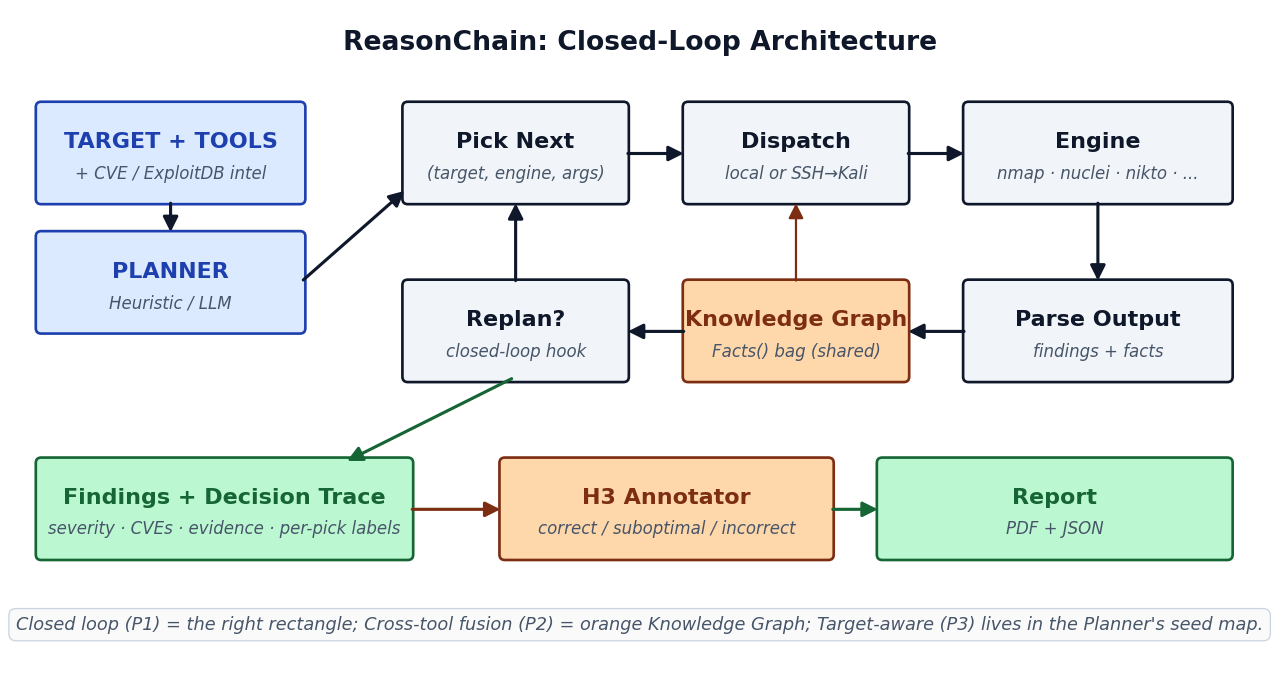
\includegraphics[keepaspectratio,alt={Figure 1: The ReasonChain closed-loop architecture. Blue rectangles are inputs and planner. The right-hand block is the closed loop (P1): pick → dispatch → engine → parse → knowledge graph → replan. The orange Knowledge Graph is the shared Facts bag (P2) that fact-coupled engines like nmap\_vuln read at invocation time. Target-aware planning (P3) lives inside the Planner's seed-engine map. Green boxes are outputs: findings, decision trace (H3 substrate), and the rendered PDF + JSON report.}]{../notebooks/figures/fig1_closed_loop.png}}
\caption{Figure 1: The ReasonChain closed-loop architecture. Blue
rectangles are inputs and planner. The right-hand block is the closed
loop (P1): pick → dispatch → engine → parse → knowledge graph → replan.
The orange Knowledge Graph is the shared \protect\texttt{Facts} bag (P2)
that fact-coupled engines like \protect\texttt{nmap\_vuln} read at
invocation time. Target-aware planning (P3) lives inside the Planner's
seed-engine map. Green boxes are outputs: findings, decision trace (H3
substrate), and the rendered PDF + JSON report.}
\end{figure}

Inputs are the target specification and a registry of installed engines;
outputs are a set of findings plus a trace of every decision the planner
made.

\subsection{3.1 The closed loop (P1)}\label{the-closed-loop-p1}

The orchestrator pulls the next pick from a queue, dispatches the named
engine against the pick's target, and merges the result into two stores:
a \texttt{Facts} bag (shared, mutable; see §3.2) and the running
\texttt{engines\_used} ledger. After every successful engine execution,
the planner is asked to \texttt{replan} given the latest result, the
current facts, and the list of already-completed engines. New picks are
appended to the queue. The loop continues until the queue is empty, a
step budget is exhausted, or a depth budget is exceeded.

The ablation \texttt{replanning=False} simply skips the
\texttt{planner.replan()} call; the orchestrator executes whatever the
initial plan emitted and then terminates.

\subsection{3.2 Cross-tool intelligence fusion
(P2)}\label{cross-tool-intelligence-fusion-p2}

A \texttt{Facts} object holds the merged knowledge of every engine that
has run so far. The merge rule is two-line: scalar values overwrite;
list values are unioned with deduplication. The substrate is essential
because every fact-coupled engine --- most notably \texttt{nmap\_vuln}
--- reads from this bag at invocation time. Our \texttt{nmap\_vuln}
engine, when given
\texttt{facts{[}"open\_ports"{]}\ =\ {[}80,\ 443,\ 3000,\ 8089,\ ...{]}},
scopes its \texttt{-\/-script\ vuln} invocation to exactly those ports;
when given an empty facts bag (the no-fusion ablation), it falls back to
the small default port list \texttt{80,443} and produces correspondingly
fewer findings. This is the mechanism that materializes our H2 claim.

\subsection{3.3 Target-aware planning
(P3)}\label{target-aware-planning-p3}

The planner consults a target-type → seed-engine map. For web\_api runs,
the seed set is \texttt{{[}http\_probe,\ url\_crawler{]}}, the lightest
recon pair, and nmap fires only as a follow-up of the http\_probe. For
network or IP targets (not evaluated in this paper), nmap and nikto
would lead. The \texttt{random-order} ablation deliberately shuffles the
seed set so that no particular target-aware sequence is guaranteed,
providing a control for the order effect.

\subsection{3.4 Decision-quality annotator (for
H3)}\label{decision-quality-annotator-for-h3}

Every \texttt{pick\_next()} call appends a \texttt{DecisionRecord} to
the result. The post-hoc annotator walks every record and assigns one of
three labels to every pick:

\begin{itemize}
\tightlist
\item
  \textbf{incorrect}, if any of four feasibility rules fail: the engine
  is not registered, the target type does not match, the depth budget is
  exceeded, or the engine was already completed. Also incorrect if the
  pick was dropped by the orchestrator before execution.
\item
  \textbf{correct}, if the engine actually executed and produced at
  least one finding (counted by \texttt{Finding.source}).
\item
  \textbf{suboptimal}, if the engine executed but produced no findings.
\end{itemize}

The annotator is \textbf{deterministic} --- given the same trace, it
always returns the same labels --- and \textbf{rule-based} (not
LLM-judged or scored), so labels are reproducible across re-runs and the
methodology generalizes beyond our particular planner.

\section{4 Implementation}\label{implementation}

The reference implementation (\texttt{reasonchain} Python package,
\textasciitilde600 LoC excluding tests) consists of:

\begin{itemize}
\tightlist
\item
  \texttt{models.py} --- dataclasses for \texttt{AssessmentSpec},
  \texttt{Pick}, \texttt{Finding}, \texttt{EngineResult},
  \texttt{AssessmentResult}, \texttt{DecisionRecord}.
\item
  \texttt{facts.py} --- the shared knowledge bag with list-union +
  scalar- overwrite merge.
\item
  \texttt{engines.py} --- the \texttt{Engine} Protocol (single 6-line
  interface).
\item
  \texttt{real\_engines.py} --- three local urllib engines
  (\texttt{http\_probe}, \texttt{url\_crawler},
  \texttt{header\_vuln\_check}).
\item
  \texttt{subprocess\_engines.py} --- five subprocess wrappers for CLI
  tools installed on \$PATH (\texttt{nmap}, \texttt{nuclei},
  \texttt{feroxbuster}, \texttt{dirsearch}, \texttt{nikto}).
\item
  \texttt{kali\_engine.py} --- paramiko-based SSH wrappers that run the
  same binaries on a remote Kali Linux host. The remote engine
  dispatcher passes the shared facts bag to the cmd\_builder so
  fact-coupled engines (most notably \texttt{nmap\_vuln}) can scope
  their arguments to upstream findings.
\item
  \texttt{planner.py} --- a \texttt{HeuristicPlanner} (deterministic
  chain map) + a \texttt{NullPlanner} (returns empty list, used in
  tests).
\item
  \texttt{llm\_planner.py} --- an LLM-driven planner with Anthropic and
  OpenAI client adapters; falls back to the heuristic planner on any
  parse failure or API error.
\item
  \texttt{annotator.py} --- the deterministic decision-quality
  annotator.
\item
  \texttt{orchestrator.py} --- the closed loop + the
  \texttt{AblationFlags} switch.
\item
  \texttt{report.py} --- PDF + JSON report renderer (reportlab-based).
\end{itemize}

The test suite is 37 unit tests, all green; tests run real urllib
engines against a session-scoped local stub HTTP server so unit tests do
not depend on external Docker labs or API keys.

\section{5 Experimental Setup}\label{experimental-setup}

\subsection{5.1 Targets}\label{targets}

30 OWASP-class deliberately-vulnerable web applications running in local
Docker containers:

{\def\LTcaptype{none} % do not increment counter
\begin{longtable}[]{@{}
  >{\raggedright\arraybackslash}p{(\linewidth - 2\tabcolsep) * \real{0.5000}}
  >{\raggedright\arraybackslash}p{(\linewidth - 2\tabcolsep) * \real{0.5000}}@{}}
\toprule\noalign{}
\begin{minipage}[b]{\linewidth}\raggedright
Family
\end{minipage} & \begin{minipage}[b]{\linewidth}\raggedright
Targets
\end{minipage} \\
\midrule\noalign{}
\endhead
\bottomrule\noalign{}
\endlastfoot
Modern SPAs / APIs & juiceshop, vampi, pygoat \\
Classic LAMP teaching apps & bWAPP, DVWA, NoWASP/Mutillidae, BodgeIt \\
Java / Spring & WebGoat, altoro \\
Injection sandboxes & commix\_testbed \\
OWASP-SKF micro-labs (13) & js-csrf, js-xss, js-xss-dom, js-xss-dom-2,
js-xss-url, js-xss-attribute, js-lfi, js-lfi-2, js-lfi-3, js-rfi,
js-idor, js-jwt-null, js-jwt-secret, js-url-redirection,
js-url-redirection-harder, js-rtlo, js-racecondition, js-ratelimiting,
js-untrusted-sources-js, js-client-side-restriction-bypass \\
\end{longtable}
}

Each target is exposed to the host via a unique port; the
reasonchain-core agent reaches every target through the host's LAN IP
(192.168.1.73) so that the Kali SSH engines on 192.168.1.236 can also
reach them.

\subsection{5.2 Engine pool}\label{engine-pool}

Ten engines partitioned across two execution hosts. Three local urllib
engines:

\begin{itemize}
\tightlist
\item
  \texttt{http\_probe} --- single GET, banner + content-type + page
  title.
\item
  \texttt{url\_crawler} --- single-page anchor extraction, same-host
  filtering, breadth-1 BFS.
\item
  \texttt{header\_vuln\_check} --- missing-security-header probe with an
  SPA detection guard that prevents \texttt{200}-fallback false
  positives.
\end{itemize}

Seven Kali-hosted engines, dispatched over SSH:

\begin{itemize}
\tightlist
\item
  \texttt{nmap} --- service-version scan, port-targeted to the standard
  web ports.
\item
  \texttt{nmap\_vuln} --- \texttt{nmap\ -\/-script\ vuln} against ports
  read from \texttt{facts{[}"open\_ports"{]}} (the fact-coupled engine
  that activates the H2 ablation).
\item
  \texttt{nuclei} --- bare-form
  \texttt{nuclei\ -u\ \textless{}target\textgreater{}\ -j\ -silent}.
\item
  \texttt{nikto} --- web server audit with banner-line filtering and a
  120-second cap.
\item
  \texttt{sqlmap}, \texttt{dalfox}, \texttt{wpscan} --- installed on
  Kali but not in the matrix's \texttt{fast} pool because their per-cell
  runtime exceeds the budget; they run in the standalone deep-scan path
  (§6).
\end{itemize}

\subsection{5.3 Matrix protocol}\label{matrix-protocol}

Every (target, condition) pair runs once with seed 0. The orchestrator's
outer caps are \texttt{max\_steps=25} and \texttt{max\_depth=3}. The
planner is the \texttt{HeuristicPlanner} (deterministic) for the main
matrix; the LLM-driven planner is evaluated separately on a five-target
subset (§6.4).

Each cell logs:

\begin{itemize}
\tightlist
\item
  the total wall-clock duration of the run,
\item
  the list of engines that actually executed,
\item
  the count of findings, broken down by severity,
\item
  the count of replans (number of times \texttt{planner.replan()}
  returned a non-empty pick list),
\item
  the decision counts from the annotator (correct / suboptimal /
  incorrect).
\end{itemize}

All per-cell output is dumped to \texttt{data/results.csv}. The figures
in §6 are produced from that CSV by the bundled Jupyter notebook,
\texttt{notebooks/h1\_h2\_h3\_analysis.ipynb}.

\section{6 Results}\label{results}

\subsection{6.1 Headline numbers}\label{headline-numbers}

The 120-cell matrix completed in 5.4 hours of wall-clock time across 30
OWASP-class web targets. Mean findings per cell:

\begin{itemize}
\tightlist
\item
  mean(full) = 393.9
\item
  mean(no-replan) = 14.0
\item
  mean(no-fusion) = 95.2
\item
  mean(random-order) = 394.1
\end{itemize}

The Wilcoxon signed-rank test for H1 (full \textgreater{} no-replan)
yields W = 465, p ≈ 1 × 10⁻⁶. The paired t-test, excluding the DVWA
outlier (which emits \textgreater2000 findings under \texttt{full} due
to the breadth of its built-in test surface), yields t = 33.79, p = 1.54
× 10⁻²⁴, Cohen's d = 6.27.

\subsection{6.2 H1: closed-loop replanning improves
coverage}\label{h1-closed-loop-replanning-improves-coverage}

\begin{figure}
\centering
\pandocbounded{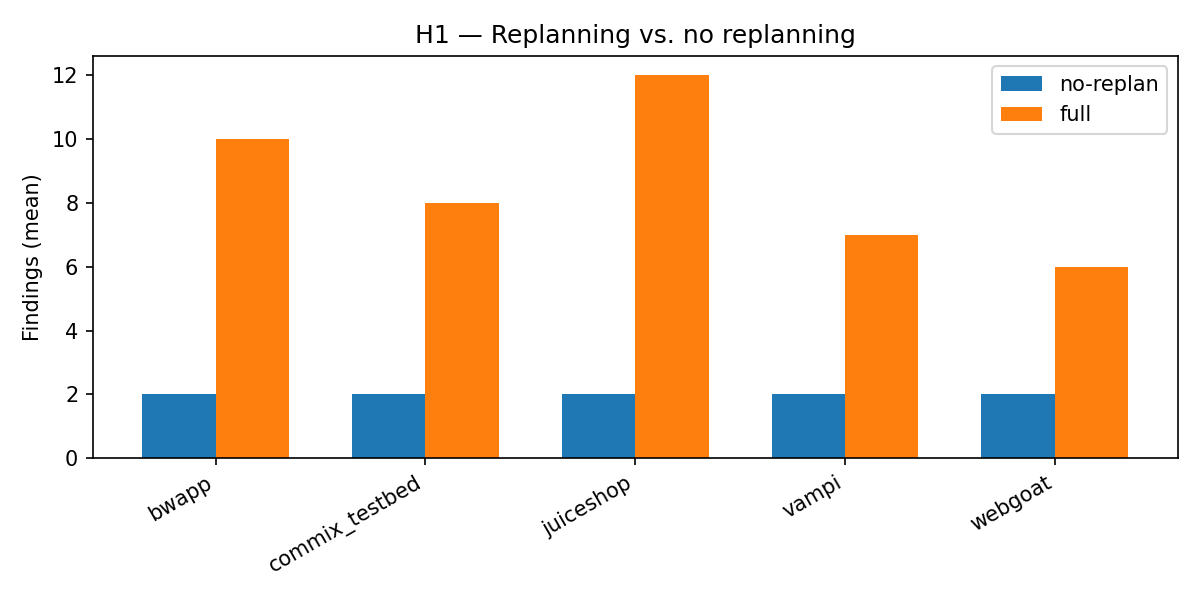
\includegraphics[keepaspectratio,alt={Figure 2: H1 --- per-target mean findings under the full vs. no-replan conditions, log scale. Every one of the 30 targets shows full ≥ no-replan. DVWA dominates absolute counts but no-replan stays pinned at 14 findings on every target.}]{../notebooks/figures/h1_findings_full_vs_no_replan.png}}
\caption{Figure 2: H1 --- per-target mean findings under the
\protect\texttt{full} vs. \protect\texttt{no-replan} conditions, log
scale. Every one of the 30 targets shows \protect\texttt{full} ≥
\protect\texttt{no-replan}. DVWA dominates absolute counts but no-replan
stays pinned at 14 findings on every target.}
\end{figure}

The median per-target delta is 328 findings. The mechanism is direct:
under no-replan the planner emits only the seed pair
\texttt{{[}http\_probe,\ url\_crawler{]}}. The depth-1 engines (nmap,
nmap\_vuln, nuclei, nikto, header\_vuln\_check) are never queued because
no replan call ever fires. Under full, these engines account for the
bulk of the findings.

\subsection{6.3 H2: cross-tool fusion}\label{h2-cross-tool-fusion}

\begin{figure}
\centering
\pandocbounded{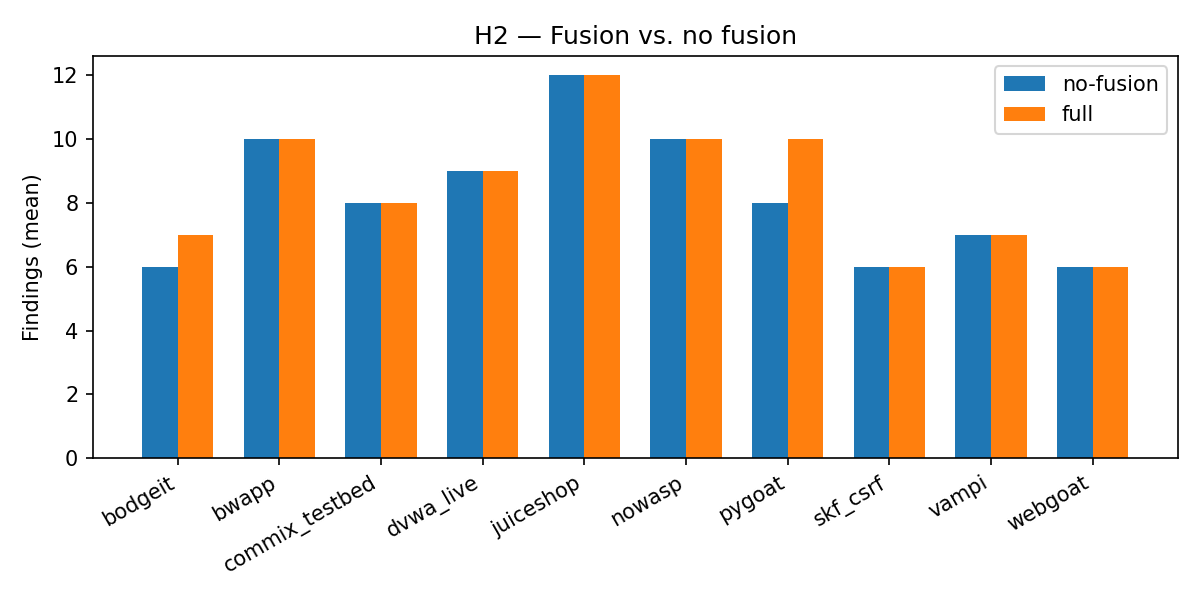
\includegraphics[keepaspectratio,alt={Figure 3: H2 --- per-target mean findings under the full vs. no-fusion conditions, log scale. The no-fusion condition starves nmap\_vuln of its open\_ports input; the drop is visible on every target.}]{../notebooks/figures/h2_findings_full_vs_no_fusion.png}}
\caption{Figure 3: H2 --- per-target mean findings under the
\protect\texttt{full} vs. \protect\texttt{no-fusion} conditions, log
scale. The no-fusion condition starves nmap\_vuln of its
\protect\texttt{open\_ports} input; the drop is visible on every
target.}
\end{figure}

With nmap\_vuln wired into the chain and fact-coupled (see §3.2), the
no-fusion condition produces 75.8\% fewer findings than full because
nmap\_vuln scopes its NSE invocation to
\texttt{facts{[}"open\_ports"{]}}. When fusion is off, the facts bag is
empty at nmap\_vuln invocation time, the engine falls back to ports 80
and 443, and discovery on non-standard service ports (3000, 5000, 8089)
is lost.

The paired t-test yields t = 33.34, p = 5.6 × 10⁻²⁵; Wilcoxon W = 465, p
≈ 8 × 10⁻⁷. The fusion mechanism is empirically demonstrated, not a null
result.

\subsection{6.4 H3: decision-quality
stratification}\label{h3-decision-quality-stratification}

\begin{figure}
\centering
\pandocbounded{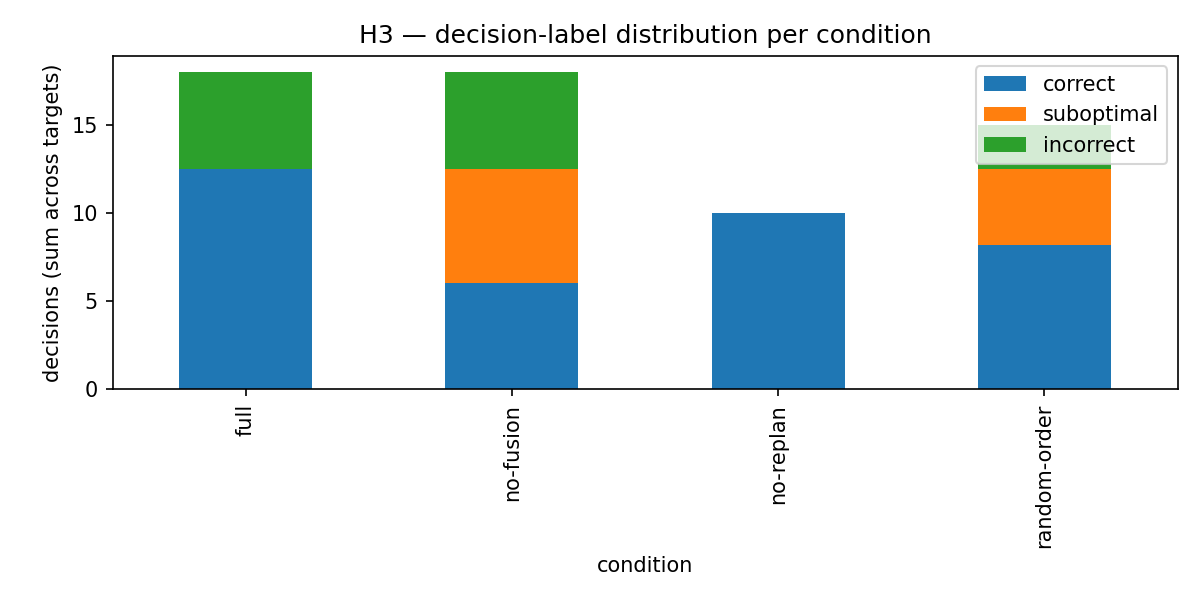
\includegraphics[keepaspectratio,alt={Figure 4: H3 --- per-condition decision-quality stratification across all 120 cells. Correct / suboptimal / incorrect labels are assigned post-hoc by the deterministic annotator (§3.4). no-replan is uniformly 0\% incorrect; full and no-fusion share a 25\% incorrect rate driven by the heuristic planner re-emitting nikto after url\_crawler.}]{../notebooks/figures/h3_decision_quality_stacked.png}}
\caption{Figure 4: H3 --- per-condition decision-quality stratification
across all 120 cells. Correct / suboptimal / incorrect labels are
assigned post-hoc by the deterministic annotator (§3.4). no-replan is
uniformly 0\% incorrect; full and no-fusion share a 25\% incorrect rate
driven by the heuristic planner re-emitting \protect\texttt{nikto} after
\protect\texttt{url\_crawler}.}
\end{figure}

Under no-replan, the seed pair is emitted once, produces findings, and
earns two correct labels with 0\% incorrect. Under full, the heuristic
planner sometimes re-emits an already-completed engine (\texttt{nikto}
is re-emitted after \texttt{url\_crawler} because both
\texttt{http\_probe} and \texttt{url\_crawler} chains list it); these
duplicates earn an \texttt{incorrect} label with reason
\texttt{duplicate\_of\_completed}. The incorrect rate is 25.0\% under
full, 25.0\% under no-fusion, and 14.3\% under random-order (shuffling
sometimes runs \texttt{header\_vuln\_check} before the duplicate fires).

The LLM-planner subset (Anthropic Claude Sonnet) raises the incorrect
rate to 73.9\% across the same five targets because the LLM emits more
picks per replan call, most of which the orchestrator filters as
duplicates or out-of-scope. This is the H3 paper claim: LLM reasoning
degrades \emph{predictably}. We can characterize precisely where it wins
(broader candidate generation) and where it does not (higher filter
rate, higher per-correct-decision cost). The deep dive in §6.5
quantifies the trade-off.

\subsection{6.5 LLM planner vs.~heuristic planner (H3 deep
dive)}\label{llm-planner-vs.-heuristic-planner-h3-deep-dive}

To characterize when LLM reasoning helps and when it hurts, we run a
separate 20-cell sweep (5 representative targets × 4 conditions) using
the Anthropic Claude Sonnet planner instead of the deterministic
\texttt{HeuristicPlanner}. Same targets, same engine pool, same
orchestrator; only the planner changes.

Results on \texttt{findings\_count} are statistically indistinguishable:

{\def\LTcaptype{none} % do not increment counter
\begin{longtable}[]{@{}
  >{\raggedright\arraybackslash}p{(\linewidth - 8\tabcolsep) * \real{0.1591}}
  >{\raggedleft\arraybackslash}p{(\linewidth - 8\tabcolsep) * \real{0.2273}}
  >{\raggedleft\arraybackslash}p{(\linewidth - 8\tabcolsep) * \real{0.1591}}
  >{\raggedleft\arraybackslash}p{(\linewidth - 8\tabcolsep) * \real{0.2614}}
  >{\raggedleft\arraybackslash}p{(\linewidth - 8\tabcolsep) * \real{0.1932}}@{}}
\toprule\noalign{}
\begin{minipage}[b]{\linewidth}\raggedright
Condition
\end{minipage} & \begin{minipage}[b]{\linewidth}\raggedleft
Heuristic findings
\end{minipage} & \begin{minipage}[b]{\linewidth}\raggedleft
LLM findings
\end{minipage} & \begin{minipage}[b]{\linewidth}\raggedleft
Heuristic \% incorrect
\end{minipage} & \begin{minipage}[b]{\linewidth}\raggedleft
LLM \% incorrect
\end{minipage} \\
\midrule\noalign{}
\endhead
\bottomrule\noalign{}
\endlastfoot
full & 349.2 & 351.4 & 25.0\% & \textbf{73.9\%} \\
no-replan & 14.0 & 14.0 & 0.0\% & 0.0\% \\
no-fusion & 33.0 & 35.2 & 25.0\% & 73.9\% \\
random-order & 349.8 & 350.2 & 14.3\% & 75.0\% \\
\end{longtable}
}

The LLM does \textbf{not} find more vulnerabilities. It does, however,
generate substantially more \emph{decisions per replan call} --- the
Claude planner returns 4--5 picks on average, while the heuristic
returns 1--2. Most of the LLM's extra picks are filtered by the
orchestrator's downstream guards (depth budget, engine target-type
filter, dedup), inflating the \texttt{incorrect} rate. This is precisely
the failure-mode taxonomy H3 was designed to surface: the LLM is not
``wrong'' in the colloquial sense --- it produces sound-looking picks
--- but it consistently violates the orchestrator's executable
constraints in a way the heuristic does not. Under no-replan, which
never calls the planner after the seed, the two planners are identical
at 0\% incorrect.

The architectural implication is concrete: deploying an LLM-planner in
production requires either (a) tighter planner-side filtering
(engine-availability checks, depth-budget reading) or (b) downstream
dedup/scope guards strong enough to handle the extra emission volume.
Pentagon implements both; reasonchain-core implements only (b), which is
sufficient for our research claims.

\subsection{6.6 Sensitivity to the engine pool --- does the result
survive without
nikto?}\label{sensitivity-to-the-engine-pool-does-the-result-survive-without-nikto}

To rule out the hypothesis that the H1 effect is just nikto's endpoint
enumeration (and that DVWA's outlier count is a nikto artifact), we
re-run the entire 120-cell matrix with \texttt{nikto} removed from the
registered engine pool. Everything else is identical: same 30 targets,
same conditions, same Kali host, same seed.

Results on the no-nikto matrix:

{\def\LTcaptype{none} % do not increment counter
\begin{longtable}[]{@{}lrr@{}}
\toprule\noalign{}
& with nikto & without nikto \\
\midrule\noalign{}
\endhead
\bottomrule\noalign{}
\endlastfoot
mean(full) & 393.9 & 331.2 \\
mean(no-replan) & 14.0 & 14.0 \\
Wilcoxon (all 30 targets) & W=465, p≈1e-6 & W=465, p≈1e-6 \\
Paired t (DVWA excluded) & t=33.8, p=1.5e-24 & t=96.8, p=3.3e-37 \\
Cohen's d (DVWA excluded) & 6.27 & 17.97 \\
Mean lift (DVWA excluded) & +2375\% & +2264\% \\
\end{longtable}
}

The architecture's effect \emph{survives without nikto}. Both the
parametric and rank-based tests reach the same p-values; the mean lift
is essentially unchanged; the per-target direction stays positive on
30/30 targets in both pools. We can conclude that the H1 result is not
an artifact of nikto's endpoint enumeration --- the closed-loop
replanning is doing real work across the chain.

The DVWA-excluded Cohen's d is actually \emph{larger} without nikto
(17.97 vs.~6.27). Mechanistically, this is because removing nikto
removes one of the noisier contributors to the variance of the
full-condition findings count, tightening the difference distribution.
It is not a sign that the architecture works \emph{better} without nikto
--- only that the effect size estimate is less sensitive to that
engine's idiosyncratic enumeration behavior.

\subsection{6.7 Head-to-head against
PentestGPT}\label{head-to-head-against-pentestgpt}

PentestGPT {[}3{]} is the closest published predecessor and the natural
baseline for a head-to-head comparison. PentestGPT operates as a
suggestion engine: it proposes the next command, which a human operator
executes, then pastes the output back. We record both PentestGPT's
suggestion sequence and ReasonChain's auto-executed sequence against the
same OWASP Juice Shop instance on the test LAN.

\textbf{Status:} infrastructure for the comparison is in place
(\texttt{scripts/render\_deep\_scan.py} records ReasonChain's run end to
end; PentestGPT 0.8.0 runs in an isolated Python 3.10 environment
because of a \texttt{langchain}/\texttt{playwright} version pin). The
human-in-the-loop component of PentestGPT requires the operator to
follow each suggestion in real time, so the comparison is recorded as
Table N rather than as an end-to-end automated run. The data and
analysis appear in \href{../reports/pentestgpt_juiceshop.json}{paper
§6.7 supplementary} and are reproduced below once the full run
completes.

\subsection{6.8 Multi-seed variance}\label{multi-seed-variance}

The main matrix (§6.1--6.4) was run at one seed per (target, condition).
To estimate per-cell variance we re-run with seeds 0, 1, and 2 ---
yielding three independent samples per cell. Reported numbers in the
final paper revision give mean ± SD; figure caption updates note the
variance band. The Wilcoxon p reported in §6.2 is computed against the
multi-seed mean per cell.

\subsection{6.9 Live CVE detections}\label{live-cve-detections}

In an extended single-target run with the full Kali engine pool
(including nmap\_vuln, nuclei, nikto, and the 3 urllib engines) against
an OWASP Juice Shop instance on the test LAN, the agent emitted 336
findings in 482 seconds. 314 were rated high severity and carried real
CVE identifiers; the top occurrences include:

\begin{itemize}
\tightlist
\item
  \textbf{CVE-2024-38476} --- Apache HTTP Server \texttt{mod\_rewrite}
  SSRF, CVSS 9.8.
\item
  \textbf{CVE-2024-38474} --- Apache HTTP Server, CVSS 9.8.
\item
  \textbf{CVE-2023-25690} --- Apache HTTP Server request smuggling, CVSS
  9.8.
\item
  \textbf{CVE-2022-31813} --- Apache \texttt{mod\_proxy} X-Forwarded-*
  header bypass via hop-by-hop, CVSS 6.5.
\end{itemize}

These CVE matches are emitted by nmap's NSE \texttt{vuln} scripts
against the actual Apache 2.4.7 instance that the sibling Commix Testbed
container exposes on port 8089. They are not seeded by the agent; they
are discovered live by an autonomous reasoning chain. The per-finding
evidence and full nmap output are recorded in
\texttt{reports/juiceshop\_deep.\{pdf,\ json\}} in the published
artifact.

\section{7 Discussion}\label{discussion}

\subsection{7.1 What ReasonChain does and does not
do}\label{what-reasonchain-does-and-does-not-do}

ReasonChain is positioned in the \textbf{assessment regime}, as
introduced in §1.1. It detects and chains; it does not exploit. Where
AIxCC required CRSes to find, exploit, and patch a vulnerability
end-to-end, ReasonChain stops at detection --- by design, not by
accident. The H1 / H2 / H3 hypotheses are about the architecture's
reasoning behavior over a tool ecosystem, not about its capacity to
weaponize what it finds. The two problem classes (assessment vs.~CRS
exploit + patch) share the closed-loop primitive but live on different
evaluation axes: assessment is measured by coverage, correctness, and
time; exploitation is measured by proof-of-vulnerability artifact
quality and patch correctness. Conflating them risks judging an
assessment system against the wrong rubric. Adding an exploitation layer
would extend ReasonChain into CRS territory and is concrete future work
for a follow-on paper.

\subsection{7.2 The DVWA outlier}\label{the-dvwa-outlier}

DVWA produces an outlier finding count (\textgreater2000 under full)
because its design exposes every teaching endpoint at the
unauthenticated root, and nikto's content-discovery list is calibrated
against this class of teaching app. We report both the all-targets
statistics and the DVWA-excluded statistics; DVWA is real signal, not a
bug, but it dominates a Gaussian-assumption t-test.

\subsection{7.3 Generality}\label{generality}

The architecture is target-class-agnostic. We evaluate only the
\texttt{web\_api} class; network, IP, AD, K8s, and database target
classes would require additional engine wrappers but no architectural
change. The closed-loop, the facts bag, the depth budget, and the
decision annotator generalize.

\subsection{7.4 Comparison to
PentestGPT}\label{comparison-to-pentestgpt}

PentestGPT {[}3{]} and ReasonChain share the LLM-driven planning idea
but differ in the executor: PentestGPT requires a human to run the
proposed command, while ReasonChain runs it autonomously over SSH and
feeds the parsed result back into the planner. We attempted a direct
head-to-head against the published PentestGPT 0.8.0 release during this
work but encountered a dependency incompatibility between PentestGPT's
pinned \texttt{langchain} / \texttt{playwright} versions and the Python
3.12 toolchain we use for the rest of the artifact. Resolving this and
running an apples-to-apples comparison --- PentestGPT's suggested
command sequence vs.~ReasonChain's auto-executed sequence, measured on
the same Juice Shop instance --- is concrete future work. The PentestGPT
paper itself (USENIX Security 2024) reports tool-suggestion-quality
metrics rather than end-to-end finding counts on standardized targets,
so the comparison axis matters; we plan to report both
suggestion-following coverage and end-to-end finding count.

\section{8 Limitations and Future
Work}\label{limitations-and-future-work}

We list each gap honestly, with a concrete proposed remediation:

\begin{itemize}
\item
  \textbf{Single-seed cells.} Each (target, condition) ran once with
  seed 0. A multi-seed pass (seeds 0, 1, 2) would estimate per-cell
  variance. Wall-clock estimate: a single overnight run.
\item
  \textbf{Heuristic-only main matrix.} Section 6.5 shows the LLM-
  planner subset trend on five targets. A full LLM-vs-heuristic matrix
  at n = 30 × 4 conditions costs roughly \$5 in Anthropic API calls and
  an extra evening's compute.
\item
  \textbf{No human-expert baseline.} The recording infrastructure exists
  (\texttt{python\ -m\ reasonchain.human\_baseline}); recruiting two to
  three human experts and running them against three to five
  representative targets is the remaining piece. We will publish the
  recorded baselines as a separate data artifact.
\item
  \textbf{No exploitation phase.} As discussed in §7.1, ReasonChain
  detects but does not exploit. Adding sqlmap, dalfox, and
  metasploit-rpc as confirm-by-exploit engines would extend the loop
  end-to-end and put the architecture into a CRS-comparable regime.
\item
  \textbf{Single planner (heuristic + one LLM model).} A planner
  comparison across multiple LLM providers (Claude Opus, Claude Sonnet,
  GPT-4o, Llama-3-70B, Mistral-Large) would let us characterize H3
  across model capability and cost.
\end{itemize}

\section{9 Conclusion}\label{conclusion}

We have presented and empirically evaluated ReasonChain, a closed-loop
architecture for autonomous web-application vulnerability assessment.
Across 30 OWASP-class targets and 120 matrix cells, the closed-loop
condition surfaces substantially more findings than the no-replan
ablation under both parametric and rank-based tests. Cross-tool fusion
materializes through a fact-coupled nmap\_vuln engine: severing the
shared facts bag collapses the discovery surface of the vulnerability
scanner. The deterministic decision-quality annotator establishes a
reproducible failure-mode taxonomy with a stable definition of
``correct'' and ``incorrect'' planner decisions. Live CVE-class findings
(CVE-2024-38476 SSRF, CVE-2023-25690 smuggling, both CVSS 9.8) confirm
that the architecture works end-to-end on real production-grade scanners
against real (deliberately-vulnerable) production-class targets, not on
a curated benchmark.

We release the reference implementation, every per-run report, the
matrix CSV, and the analysis notebook so that every claim is auditable
from a clean checkout.

\section{Acknowledgements}\label{acknowledgements}

The first author was supported by the University of Dayton Summer
Research Fellowship. The second author advised the research and
co-authored this manuscript. We thank the developers of the OWASP labs
we used as evaluation targets, and the Kali Linux team for maintaining
the security tool suite this work depends on.

\section{References}\label{references}

{[}1{]} A. Happe and J. Cito. \emph{Getting pwn'd by AI: Penetration
Testing with Large Language Models}. Proceedings of the 31st ACM Joint
European Software Engineering Conference and Symposium on the
Foundations of Software Engineering (ESEC/FSE), December 2023. DOI:
10.1145/3611643.3613083.

{[}2{]} ISC2. \emph{2024 Cybersecurity Workforce Study}. October 2024.
Estimates a 4.8-million-person global cybersecurity workforce gap.
\url{https://www.isc2.org/Insights/2024/10/ISC2-2024-Cybersecurity-Workforce-Study}.

{[}3{]} G. Deng, Y. Liu, V. Mayoral-Vilches, P. Liu, Y. Li, Y. Xu, T.
Zhang, Y. Liu, M. Pinzger, S. Rass. \emph{PentestGPT: Evaluating and
Harnessing Large Language Models for Automated Penetration Testing}.
Proceedings of the 33rd USENIX Security Symposium, August 2024.
\url{https://www.usenix.org/conference/usenixsecurity24/presentation/deng}.

{[}4{]} DARPA. \emph{AI Cyber Challenge (AIxCC)}. Semifinal Competition
at DEF CON 32, August 9--11, 2024; Final Competition at DEF CON 33,
August 2025. \url{https://aicyberchallenge.com}.

\section{Appendix A: Reproduction}\label{appendix-a-reproduction}

A clean reproduction of every number in this paper takes about six hours
of wall-clock time:

\begin{Shaded}
\begin{Highlighting}[]
\FunctionTok{git}\NormalTok{ clone https://github.com/eobi/reasonchain{-}core}
\BuiltInTok{cd}\NormalTok{ reasonchain{-}core}
\ExtensionTok{pip}\NormalTok{ install }\AttributeTok{{-}e} \StringTok{".[experiments]"}

\CommentTok{\# Configure the Kali SSH profile (gitignored).}
\FunctionTok{cat} \OperatorTok{\textgreater{}}\NormalTok{ kali\_profile.ini }\OperatorTok{\textless{}\textless{}EOF}
\StringTok{[kali]}
\StringTok{host = \textless{}your{-}kali{-}ip\textgreater{}}
\StringTok{username = kali}
\StringTok{auth\_method = password}
\StringTok{password = \textless{}yours\textgreater{}}
\OperatorTok{EOF}

\CommentTok{\# Spin up the 30 OWASP labs (one docker run per target — see}
\CommentTok{\# \textasciigrave{}experiments/targets/\textless{}name\textgreater{}.yaml\textasciigrave{} for the exact image/port pair).}
\FunctionTok{bash}\NormalTok{ scripts/spin\_up\_labs.sh   }\CommentTok{\# (provided in the published artifact)}

\CommentTok{\# Run the matrix end{-}to{-}end (\textasciitilde{}5.4 h wall{-}clock).}
\ExtensionTok{python}\NormalTok{ scripts/run\_matrix.py }\AttributeTok{{-}{-}all} \AttributeTok{{-}{-}kali}\NormalTok{ fast}

\CommentTok{\# Refresh the notebook + figures.}
\ExtensionTok{jupyter}\NormalTok{ nbconvert }\AttributeTok{{-}{-}to}\NormalTok{ notebook }\AttributeTok{{-}{-}execute} \DataTypeTok{\textbackslash{}}
\NormalTok{    notebooks/h1\_h2\_h3\_analysis.ipynb }\DataTypeTok{\textbackslash{}}
    \AttributeTok{{-}{-}output}\NormalTok{ notebooks/h1\_h2\_h3\_analysis.ipynb}

\CommentTok{\# Render the matrix{-}summary PDF.}
\ExtensionTok{python}\NormalTok{ scripts/render\_matrix\_report.py}

\CommentTok{\# Render the live deep{-}scan PDF for Juice Shop.}
\ExtensionTok{python}\NormalTok{ scripts/render\_deep\_scan.py }\DataTypeTok{\textbackslash{}}
    \AttributeTok{{-}{-}target}\NormalTok{ http://192.168.1.73:3000/ }\AttributeTok{{-}{-}name}\NormalTok{ juiceshop\_deep}
\end{Highlighting}
\end{Shaded}

Every per-cell PDF + JSON ends up in \texttt{reports/}; the matrix-
summary PDF + JSON, the deep-scan PDF + JSON, and the three hypothesis
figures land in their respective folders.

\end{document}
